\documentclass[a4paper,12pt]{book}
\usepackage{CJKutf8}
\usepackage{titlesec}
\usepackage{graphicx} 
\usepackage{subfigure}
\usepackage{amsbsy}
\usepackage{amsmath}
\usepackage{amssymb}
\usepackage{array}
\usepackage[colorlinks,linkcolor=blue]{hyperref}
\usepackage{enumitem}
\newtheorem{definition}{Definition}


\begin{CJK}{UTF8}{gbsn}
    %%*****************文本设置********************
    \RequirePackage{indentfirst}
    \setlength{\parindent}{2em}
    %% 行距
    \linespread{1.3}
    \selectfont
    % 页面顶行空白
    \setlength{\topskip}{5ex}
    % 段间距
    \setlength{\parskip}{1ex}
    %item 的缩进%
    \setlength{\itemindent}{2em}
    %%********************************************
    

    \begin{document}
    \title{机器学习基础笔记}
    \author{Kevin}
    \date{2020-06-22}
    \maketitle

    \newpage
    \tableofcontents

    \chapter{线性建模——最小二乘法}
    \section{写在最前}
    讨论这个方法之前,先说些题外话。
    首先,我感觉机器学习是一门值得我们去了解和学习的一门技术,
    它不仅仅应用于我们的生活,而且不断地在改变着我们的方方面面。
    虽然很早就已经接触它,并开始学习,但是总体感觉是学习的比较混乱,
    仅以从今天开始的一系列文章作为重新总结和学习机器学习的一个新的历程。
    其次,学习机器学习,要有耐心,要执着,要不断总结和实现。
    最后,也是最重要的,要明白你的初衷是什么,也就是为什么要学习它。
    如果没有搞清楚为什么,那还是先弄清楚吧。好了,废话不多说了,开始进入正题。
    
    \section{引言}
    机器学习中的一个大类的问题就是分类问题。分类在我们的生活中也是很常见的,
    比如说,你刚进入大学,要分清哪些同学喜欢玩游戏,哪些喜欢学习,
    这样,你想玩游戏的时候可以找爱玩游戏的同学一起,你学习遇到难题可以找
    喜欢学习的同学请教。
    
    
    当然,你的好友可以同时做到以上两点那是最好不过的了。
    还要提一下
    \textbf{分类和回归的区别},
    当我们要解决的问题是预测的离散值的时候,也就是上面提到的例子,
    分清哪些人喜欢玩游戏,哪些人喜欢学习,这就是一个分类问题。
    当要预测的值是一个连续值的话,那这就是一个回归问题。
    比如,我们可能在刚上大学的时候,不了解同学们平时喜欢打游戏或者喜欢学习,
    但是我们知道他们一系列的其他信息:A同学周一到周五喜欢去图书馆、自修室,
    但是周末就和寝室的同学打游戏,甚至玩通宵,当然还有其他信息。
    那么,我们的问题是A同学喜欢学习的可能性有多大,
    这个问题的答案是[0,1]上的任意一个实数(这取决于你的预测模型),
    你可能根据你的系统推测出A喜欢学习的概率是0.51。
    

    \section{问题的提出}
    我们考虑简单的单一变量的线性回归。我这里为了简便就举《机器学习基础教程》
    上的例子。男子100m比赛赢得金牌不同举办年份所需的时间。
    如图1 所示:

    \begin{figure}[h]
        \centering
        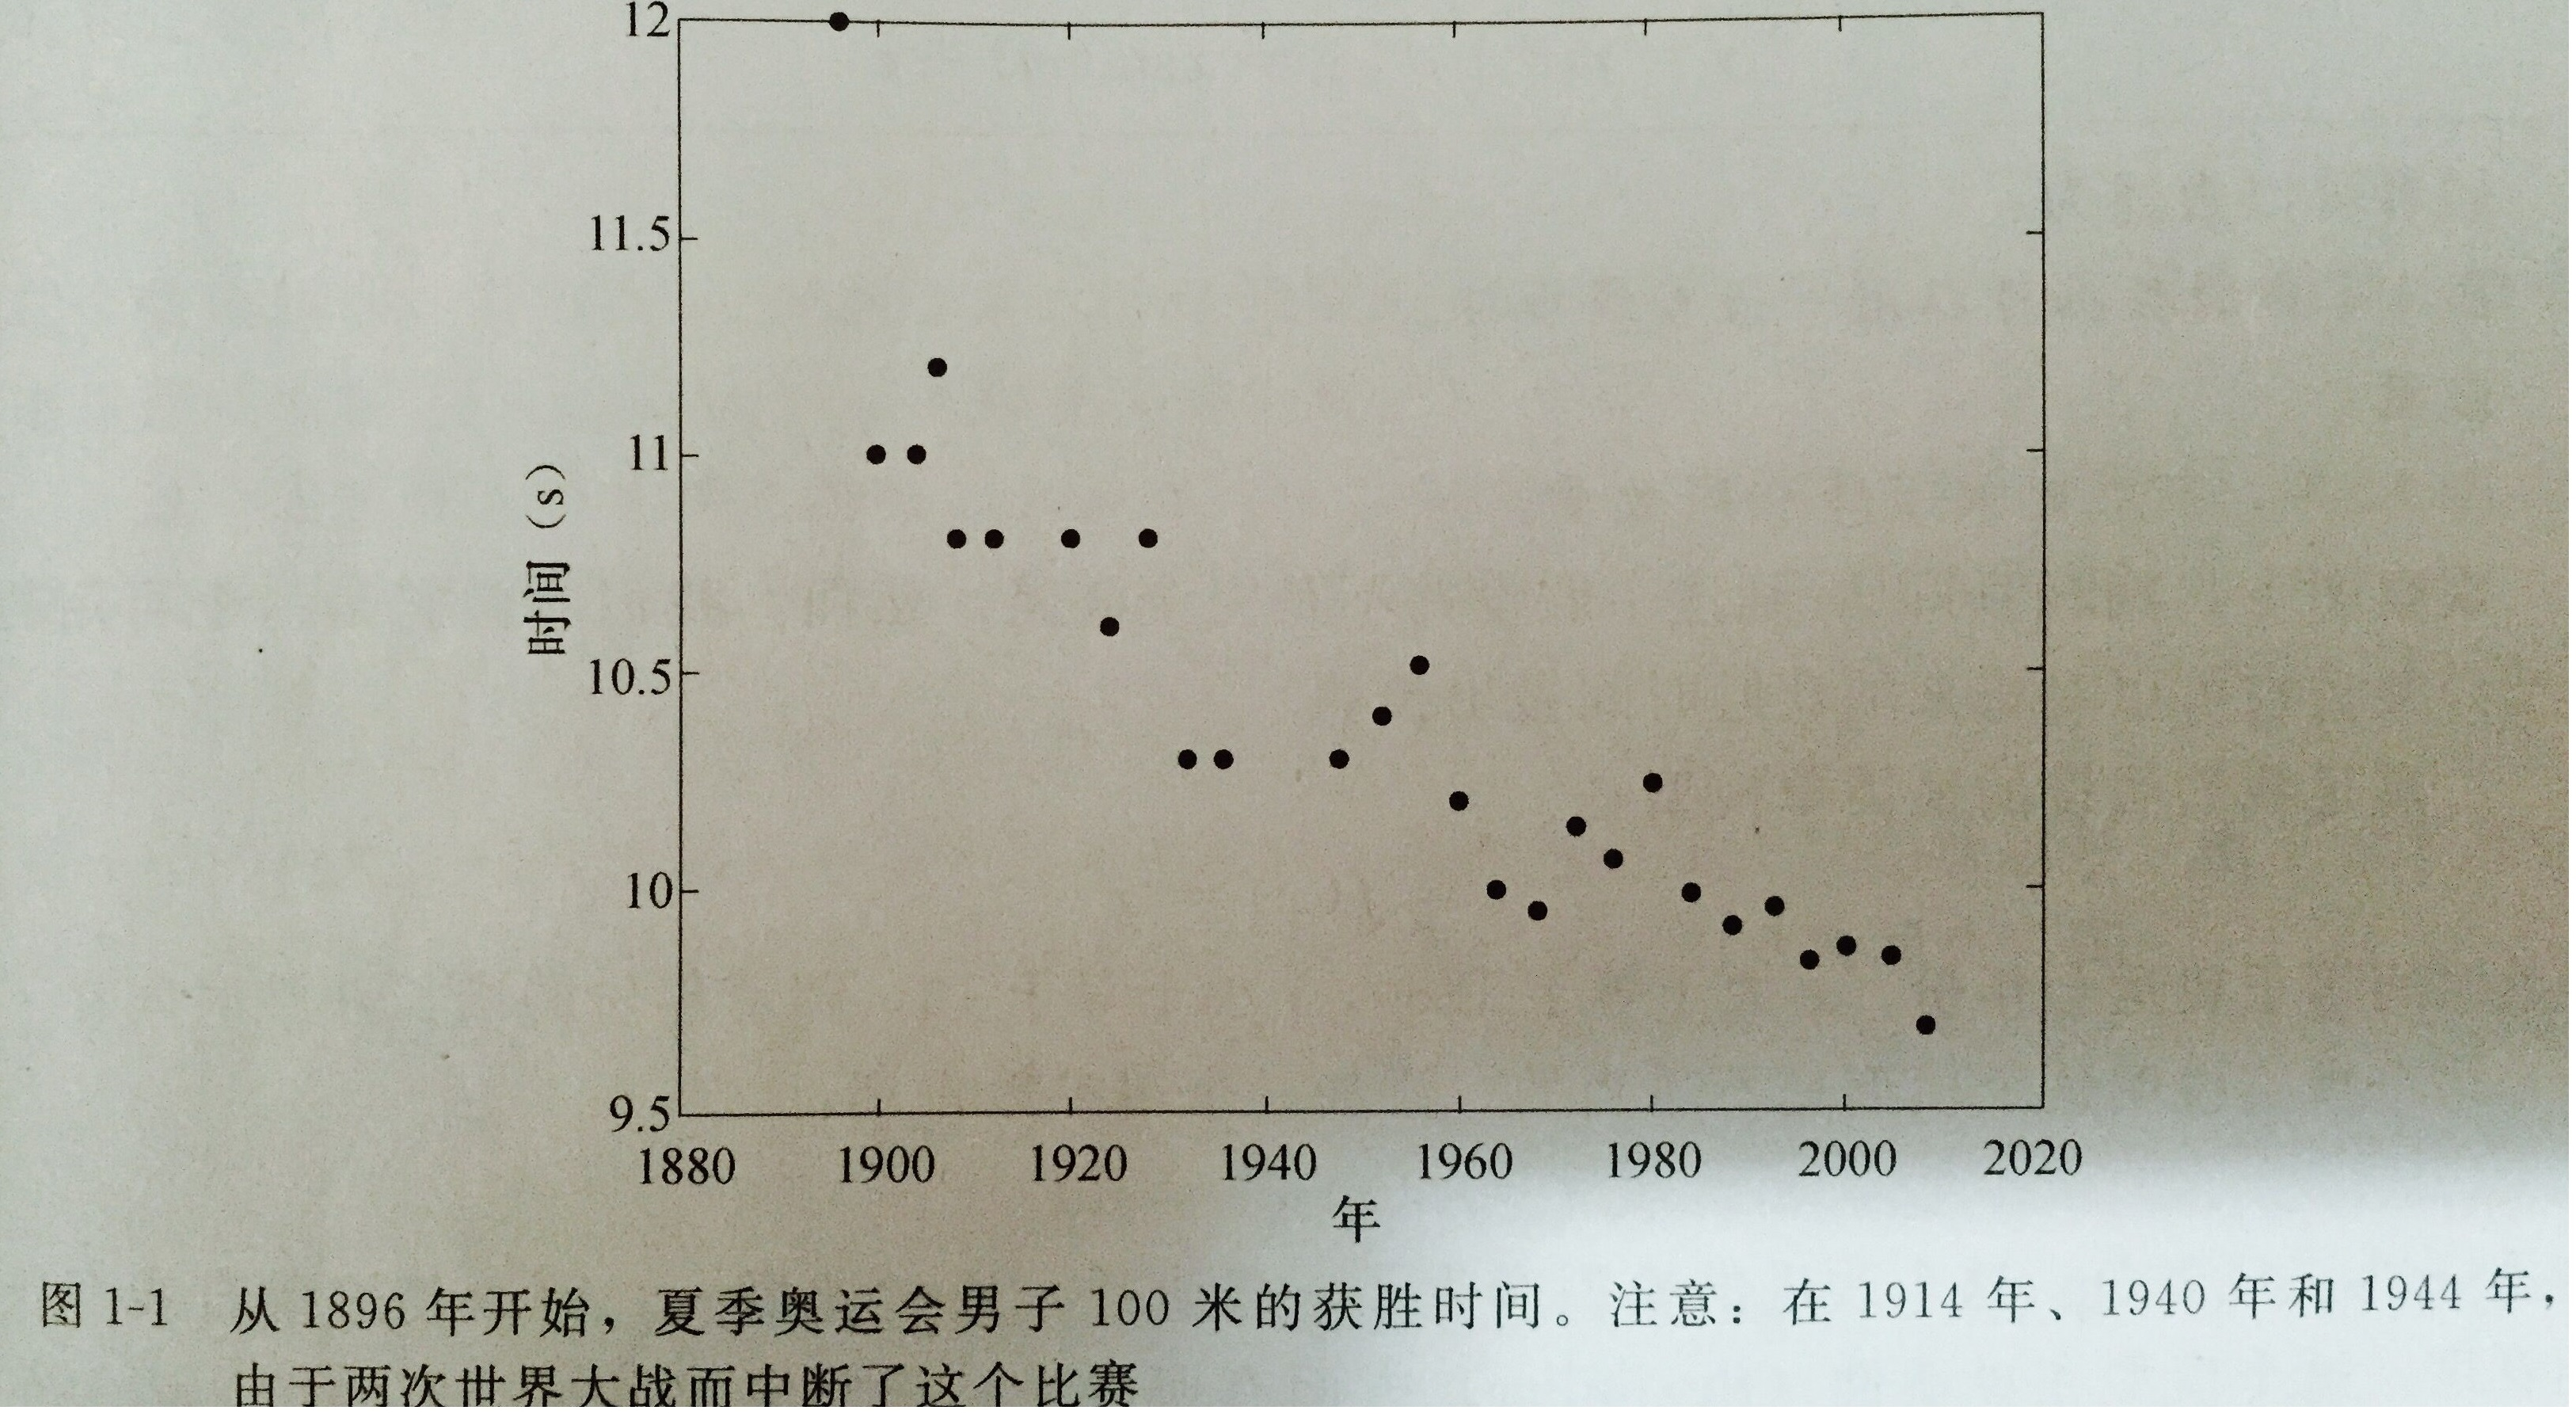
\includegraphics[width=10cm,height=7cm]{1_1}
        \caption{男子100m比赛赢得金牌所需时间数据分布}
    \end{figure}
    通过上图,我们至少可以看到年份和获胜时间存在一个关系。我们要预测2016年男子100米金牌所需的时间。

    \section{模型假设}
    $y$表示所需时间, $x$表示年份,则有如下假设。
    $$ y = ax+b \quad(1)$$


    我们现在知道2016年之前每届奥运会的男子100米金牌所需的时间,
    通过图一我们看到数据点的分布呈现一种趋势关系,
    假设它们分布在公式1所示的直线周围,我们的目标是找到一条直线,
    来拟合我们的观测数据,进而用我们找到的这条最佳的线预测2016年的男子100m金牌所需时间。
    那么,什么样的直线最好呢?我们如何求公式1中的$a$, $b$ 这两个参数呢?
    

    假定我们的模型已经选择好了,
    那么衡量这个模型的一个常用方式就是用\textbf{平方损失函数}:
    $$L(t,f(x;a,b)) = (t-f(x;a,b))^2 \quad(2)$$
    上述公式(2)最小,我们就说模型对我们现有的观测数据来说是最好的,
    我们暂且抛开数据过拟合的问题。
    那么问题转化为求$L(t,f(x;a,b))$取得最小值时候的$a,b$.令$n$代表历史数据的数目,则我们的损失函数可以写为:
    $$L=\sum_{i}^n(y_i-(ax_i+b))^2\quad(3)$$
        
    \section{推导过程}


    用公式(3)分别对$a,b$求偏导数,然后令其分别等于0, 这就可以求得$a, b$. 这里用到了函数极值,可以参考高等数学。
    $$
    \begin{array}{ll}\frac {\partial L}{\partial a} = \sum_{i}^n
    2(y_i-(ax_i+b))(-x_i)\\
    \quad=-2\sum_i^n(y_ix_i-ax_i^2-bx_i) =0 \quad (4)\\
    \frac{\partial L}{\partial b}=\sum_i^n2(y_i-(ax_i+b))(-1)\\=-2\sum_i^n(y_i-ax_i-b)=0\quad(5)
    \end{array}
    $$
    利用公式4,5求解得:
    $$
    a=\frac{\sum_i^nx_i\sum_i^ny_i-n\sum_i^ny_ix_i}
    {(\sum_i^nx_i)^2-n\sum_i^nx_i^2}
    $$
    $$
    b=\frac{\sum_i^nx_i\sum_i^ny_ix_i-\sum_i^nx_i^2\sum_i^ny_i}{(\sum_i^nx_i)^2-n\sum_i^nx_i^2}
    $$


    \section{总结}

    本文介绍了最小二乘法拟合数据的过程,最小二乘法是最优化方法中的一个,
    要了解更多优化方法,可以看看《最优化导论》。本文的事例只考虑了一个变量:年份,如果有多个自变量,它们在空间中也满足线性分布,
    能不能用最小二乘法去拟合数据呢?这个问题,我将在下一篇文章中进行介绍。
    
    \chapter{多变量最小二乘法}

    \section{引言}
    在上一节中,我们介绍了最简单的学习算法——最小二乘法去预测奥运会男子100米时间。但是可以发现,它的自变量只有一个:年份。
    通常,我们所面对的数据集往往不是单个特征,而是有成千上万个特征组成。那么我们就引入特征的向量来表示,
    这里涉及到矩阵的乘法,向量,矩阵求导等一些线性代数的知识。

    \section{将拟合函数由单变量改写为多变量}
    设我们的拟合函数 
    $$
    f(\boldsymbol{x_i}; \boldsymbol{\omega}) = \boldsymbol{\omega}^T\boldsymbol{x_i}
    $$

    其中, $\boldsymbol{w}$表示拟合函数的参数,$\boldsymbol{x_i}$表示数据集中第i条数据。

    对于上节中的$f(x;a,b) = ax + b$,我们可以令
    $$ \boldsymbol{\omega} = \begin{bmatrix}
    a\\b
    \end{bmatrix}, 
    \boldsymbol{x_i} = \begin{bmatrix}
    x\\1
    \end{bmatrix}$$

    则这两个函数等价。为了方便推导,我们在损失函数前边加上$\frac{1}{N}$,由于N是定值,它代表数据集的记录数。那么,损失函数可以写为:
    $$
    L=\frac{1}{N}\sum_{i=1}^{N}(y_i-\boldsymbol{\omega^Tx_i})^2=\frac{1}{N}(\boldsymbol{y}-\boldsymbol{X\omega})^T(\boldsymbol{y}-\boldsymbol{X\omega}) (1)
    $$
    那么上式的推导过程也很简单,令
    $$
    \boldsymbol{X}=\begin{bmatrix}
    \boldsymbol{x_1^T} \\
    \boldsymbol{x_2^T} \\
    \vdots\\
    \boldsymbol{x_n^T}
    \end{bmatrix}
    =\begin{bmatrix}
    1 & x_1\\
    1 & x_2\\
    \vdots & \vdots\\
    1 & x_n
    \end{bmatrix}
    $$

    $$
    \boldsymbol{y}=\begin{bmatrix}
    y_1\\
    y_2\\
    \vdots\\
    y_n
    \end{bmatrix}, \boldsymbol{\omega}=\begin{bmatrix}
    \omega_0\\
    \omega_1
    \end{bmatrix}
    $$

    带入(1)式即可得证,此处略过。

    \section{多特征下求解参数 \textbf{${\omega}$}}

    $$
    \begin{aligned}
    L&=\frac{1}{N}(\boldsymbol{y}-\boldsymbol{X\omega})^T(\boldsymbol{y}-\boldsymbol{X\omega}) \\
    &=\frac{1}{N}(\boldsymbol{y^T-\omega^TX^T})(\boldsymbol{y}-\boldsymbol{X\omega})\\
    &=\frac{1}{N}(\boldsymbol{y^Ty-y^TX\omega-\omega^TX^Ty+\omega^TX^TX\omega})\\
    &=\frac{1}{N}(\boldsymbol{\omega^TX^TX\omega-2\omega^TX^Ty+y^Ty})(2)
    \end{aligned}
    $$

    我们的目标是让损失函数最小,即求(2)的最小值,我们对$\boldsymbol{\omega}$求偏导数,令其等于0,就可以求出$L$取得极小值时参数$\boldsymbol{\omega}$的值。
    
    \begin{equation}
        \begin{split}
        \label{E1}
            \frac{\partial{L}}{\partial{\boldsymbol{\omega}}}=\frac{1}{N}(2\boldsymbol{X^TX\omega-2X^Ty})=0(3)\\
            \Rightarrow  \boldsymbol{X^TX\omega=X^Ty}\\
            \Rightarrow  \boldsymbol{\omega=(X^TX)^{-1}X^Ty}
        \end{split}
    \end{equation}
   
    
    至此,我们已经求出了参数值,接下来就可以预测了。至于(3)的求导,注意以下求导公式即可:
    \begin{table}[h]
        \centering  % 显示位置为中间
	    \caption{矩阵求导}  % 表格标题
	    \label{table1}  % 用于索引表格的标签
	    %字母的个数对应列数,|代表分割线
	    % l代表左对齐,c代表居中,r代表右对齐
        \begin{tabular}{|c|c|}  
            \hline  % 表格的横线
            $f(\boldsymbol{w})$&$\frac{\partial{f}}{\partial{\boldsymbol{w}}}$ \\  % 表格中的内容,用&分开,\\表示下一行
            \hline
            $\boldsymbol{w^Tx}$&$\boldsymbol{x}$ \\
            \hline
            $\boldsymbol{x^Tw}$&$\boldsymbol{x}$ \\
            \hline
            $\boldsymbol{w^Tw}$&$\boldsymbol{2w}$\\
            \hline
            $\boldsymbol{w^TCw}$&$\boldsymbol{2Cw}$\\
            \hline
        \end{tabular}
    \end{table}

    \chapter{正则化最小二乘法}
    \section{模型的泛化与过拟合}

    在上一节中,我们的预测函数为:
    $$f(x;\omega) = \omega^Tx$$
    其中,
    $$
    x=\begin{bmatrix}
    x\\
    1
    \end{bmatrix},
    \omega=\begin{bmatrix}
    \omega_1\\
    \omega_0
    \end{bmatrix}
    $$


    上述称为线性模型,我们也可以将$x$扩展为:
    $$
    x=\begin{bmatrix}
    x^n\\
    \vdots\\
    x^2\\
    x\\
    1
    \end{bmatrix},
    \omega=\begin{bmatrix}
    \omega_n\\
    \vdots\\
    \omega_2\\
    \omega_1\\
    \omega_0
    \end{bmatrix}
    $$


    那么预测函数$f(x;w)$就变为一个非线性函数。预测函数的次数越高,越能准确地拟合训练数据。在某些情况下,高次预测函数会拟合大部分或全部训练数据,这时,我们就说这个模型过拟合。因为这种过度拟合训练数据的模型对未知数据的预测就不是那么准确了,它对训练数据外的其它数据是相当敏感的,也就是说它不够泛化。所以我们需要一个最好的模型,也就是说我们需要的模型误差要最小,而且还有一定的泛化能力。
    
    \section{正则化最小二乘法}
    
    要避免模型过拟合,我们可以选择部分数据进行模型的训练,也可以利用正则化方法。一般来讲,正则化,有L1正则和L2正则,它们都是基于$L_p$范数的:
    $$L_p=(\sum_i^n\vert x_i\vert ^p)^\frac{1}{p}$$
    这里我们选择模型的复杂度为L2正则:$\sum_i^n\omega_i^2$,写为向量形式为:$\omega^T\omega$.
    
    
    关于正则化的详细内容,可以参考:
    \href{http://blog.csdn.net/heyongluoyao8/article/details/49429629}{正则化}
    
    那么我们新的损失函数可以写为:
    $$
    \begin{aligned}
    L' &= L+\boldsymbol{\lambda\omega^T\omega}\\
    &=\frac{1}{N}(\boldsymbol{\omega^TX^TX\omega-2\omega^TX^Ty+y^Ty})+\lambda\boldsymbol{\omega^T\omega}
    \end{aligned}
    $$
    同样的对上式求偏导数:
    \begin{equation}
        \begin{split}
            \label{E1}
            \frac{\partial{L}}{\partial{\boldsymbol{\omega}}}=\frac{1}{N}(2\boldsymbol{X^TX\omega-2X^Ty})+2\lambda\boldsymbol{\omega}=0\\
            \Rightarrow(\boldsymbol{X^TX}+N\lambda\boldsymbol{I})\omega=\boldsymbol{X^Ty}\\
            \Rightarrow\boldsymbol{\omega}=(\boldsymbol{X^TX}+N\lambda\boldsymbol{I})^{-1}\boldsymbol{X^Ty}
        \end{split}
    \end{equation}
    
    
    选择$\lambda$的值就是选择多项式拟合函数时,折中过拟合/泛化的过程。值太小,过拟合;值太大,不利于数据的逼近。至于$\lambda$的选择,可以采用交叉验证获得最好预测性能的$\lambda$。

    \chapter{最大似然估计}
    \section{最大似然估计的基本思想}

    最大似然估计的基本思想是:从样本中随机抽取n个样本,
    而模型的参数估计量使得抽取的这n个样本的观测值的概率最大。
    最大似然估计是一个统计方法,它用来求一个样本集的概率密度函数的参数。
    
    \section{似然估计}
    
    在讲最小二乘法的时候,我们的例子是奥运会男子100m金牌所需要的时间,
    通过最小二乘法,我们求得了我们的模型参数。
    但是我们的模型目前预测的只是一个特定的值。
    实际上,所有的模型都有误差,也就是噪声。
    所以,我们需要思考如何产生与我们观察到的数据相似的数据。
    定义新的模型如下:
    $$t_n = \boldsymbol{\omega}^T\boldsymbol{x}_n+\varepsilon_n$$
    
    假设误差$\varepsilon$是独立的、连续的、而且服从正态分布。
    即上式满足:
    $$
    \varepsilon_n \sim N(0, \sigma^2)
    $$
    给高斯随机变量添加一个常量等同于具有相同常量转换来的均值的另一个高斯随机变量:
    $$
    y = a + z \\
    p(z) = N(m, s) \\
    p(y) = N(m+a, s) \\
    $$
    
    则 $p(t_n|\boldsymbol{x_n, \omega, }\sigma^2) = N(\boldsymbol{\omega}^T\boldsymbol{x}_n, \sigma^2)$, 这里我们需要确定两个值: $\omega, \sigma^2$的最优值。
    
    对于给定的$\omega, t_n$是独立的,也就是说观测值是独立的。
    那么,整个数据集的似然值为:
    $$
    L = p(\boldsymbol{t|x_n, \omega, }\sigma^2) = \prod_{n=1}^Np(t_n|\boldsymbol{x_n, \omega, }\sigma^2) =\prod_{n=1}^NN(\boldsymbol{\omega}^T\boldsymbol{x}_n, \sigma^2)
    $$ 
    
    最大化似然值即最大化似然对数,所以上式等价于求$w 和 
    \sigma^2$的最大似然解使得$log L$最大。
    则通过求解:
    $$
    \frac{\partial{log L}}{\partial{\boldsymbol{\omega}}} = \boldsymbol{0}(1)\\
    \frac{\partial{log L}}{\partial{\sigma}}=0(2)
    $$
    
    求解的过程略过,得到$\boldsymbol{\omega}和\hat{\sigma^2}$的最大似然解:
    $$
    \boldsymbol{\hat{\omega}=(X^TX)^{-1}X^Ty}\\
    \hat{\sigma^2} = \frac{1}{N}(\boldsymbol{t}^T\boldsymbol{t}-\boldsymbol{t}^T\boldsymbol{X\hat{\omega}})
    $$
    

    求解最大似然函数的一般步骤为:

    1. 写出似然函数


    2. 写出对数似然函数,并整理
    
    
    3. 求导数
    
    
    4. 解似然方程

    
    \chapter{朴素贝叶斯}
    \section{朴素贝叶斯分类}
    \subsection{分类问题}
    分类实际上是我们在日常生活中经常使用的。比如说,在工作中,把自己手头的任务分为轻重缓急,然后按照优先级去完成它们。
    
    朴素贝叶斯法是基于贝叶斯定理与特征条件独立假设的分类方法。
    
    从数学的角度看$C=\{c_1, c_2, \dots, c_k\}$是类别的集合,集合$X=\{x_1,x_2,\dots,x_k\}$是输入集合 。这里,对于给定的输入$x$计算后验概率最大的$c$。
    
    \subsection{概率相关}
    
    由
    $$P(X,Y)=P(X|Y)P(Y)=P(Y|X)P(X)
    $$
    得
    $$
    P(Y|X) = \frac{P(X|Y)P(Y)}{P(X)} 
    $$
    
    $P(X,Y)$是$X和Y$的联合分布,训练数据集
    $$
    T=\{(x_1,y_1),(x_2,y_2),\dots,(x_n,y_n)\}
    $$
    是由$P(X,Y)$独立同分布产生的。
    
    \subsection{朴素贝叶斯方法}
    对于给定的输入$x$, 需要输出$y$,使得$P(Y=c_k|X=x)$最大。由1式可知,分母是常数,我们使分子的最大化即可。
    
    其中,$P(Y=c_k), k=1, 2, \dots, K$ 称为先验概率分布。这项可以简单的求出。
    $$P(X=x|Y=c_k)=P(X^{(1)}=x^{(1)}, \dots, X^{(n)}=x^{(n)} |Y=c_k)$$
    
    由于上式有指数型的参数,所以很难估计,为了便于计算,假设输入向量$x$的各个特征之间是条件独立的:
    \begin{equation}
        \begin{aligned}
                P(X=x|Y=c_k)&=P(X^{(1)}=x^{(1)}, \dots, X^{(n)}=x^{(n)} |Y=c_k) \\
                &=\prod_{j=1}^nP(X^{(j)}=x^{(j)}|Y=c_k)
        \end{aligned}
    \end{equation}
    
    这也是朴素贝叶斯名字的来源。
    
    则,最终结果
    
    $$y = f(x) =arg \max_{c_k}P(Y=c_k) \prod_{j=1}^nP(X^{(j)}=x^{(j)}|Y=c_k)$$
    
    \subsection{总结}
    
    朴素贝叶斯实际上是学到生成数据的机制,即它是生成模型。条件独立的假设说明分类特征是条件独立的,这个假设使得计算大大简化,但是有时也牺牲了一定的准确性。

    \section{朴素贝叶斯算法的后验概率最大化含义}
    上一节中讲了朴素贝叶斯算法将实例分到后验概率最大的类。这等价于期望风险最小化。
 
    假设使用0-1损失函数:
    $$
    L(Y, f(X)) = \Bigg\{ \begin{array} {ll}
    1,  & Y \neq f(X) \\
    0, & Y = f(X)
    \end{array}
    $$

    上式中的$f(x)$是分类决策函数, 这时,期望风险函数是:
    $$
    R_{exp}(f)=E[L(Y, f(X))]
    $$

    此期望是对联合分布$P(X, Y)$ 取的。由此取条件期望
    $$
    R_{exp}(f) = E_X \sum_{k=1}^K[L(c_k, f(X))]P(c_k|X)
    $$
    为了使期望风险最小化,只需对$X=x$逐个极小化:
    
    \begin{equation}
        \begin{aligned}
            f(x) &=arg \min_{y \in Y} \sum_{k=1}^KL(c_k,y)P(c_k|X=x) \\
            &=arg \min_{y \in Y} \sum_{k=1}^KP(c_k \neq Y|X=x) \\
            &=arg \min_{y \in Y} \sum_{k=1}^K(1-P(c_k = Y|X=x) )\\
            &=arg \max_{y \in Y} \sum_{k=1}^KP(c_k = Y|X=x) 
        \end{aligned}
    \end{equation}


    通过以上推导,根据期望风险最小化得到了后验概率最大化:
    $$
    f(x)=arg \max_{c_k}P(c_k|X=x) 
    $$
    这就是朴素贝叶斯算法所使用的原理。

    \section{朴素贝叶斯法的参数估计}
    \subsection{极大似然估计}

    在上一笔记中,经过推导,得到了朴素贝叶斯分类器的表示形式:
    > $$ y = arg \max_{c_k} P(Y=c_k)\prod_jP(X^{(j)} =  x^{(j)}| Y=c_k)  (1)$$

    也就是说,朴素贝叶斯方法的学习是对概率$P(Y=c_k)$和$P(X^{(j)} =  x^{(j)}| Y=c_k) $的估计。故可以用极大似然估计法估计上述先验概率和条件概率。
    先验概率$P(Y=c_k)$的极大似然估计为:
    $$P(Y=c_k) = \frac{\sum_{i=1}^{N}I(y_i=c_k)}{N}, k=1,2, \dots, K$$

    条件概率$P(X^{(j)} =  a_{jl}| Y=c_k) $的极大似然估计是:
    $$P(X^{(j)} =  a_{jl}| Y=c_k) = \frac{\sum_{i=1}^{N}I(x_i^{(j)} =  a_{jl},y_i=c_k)}{\sum_{i=1}^{N}I(y_i=c_k)}$$
    其中,$x_i^{(j)}$是第i个样本的第j个属性;$a_{jl}$是第j个属性可能取l的值;$I$是指示函数。
    将上述两个极大似然估计的值求出后,根据(1)式确定输入实例的分类。
    \subsection{贝叶斯估计}

    由(1)式可以得知,用极大似然估计可能导致估计出来的概率为0的情况,这会影响后验概率的计算结果,使得后验概率为0,解决这一问题的方法是采用贝叶斯估计。
    先验概率$P_{\lambda}(Y=c_k)$的贝叶斯估计是:
    $$
    P(Y=c_k) = \frac{\sum_{i=1}^{N}I(y_i=c_k)+\lambda}{N+K\lambda}
    $$

    条件概率$P_{\lambda}(X^{(j)} =  a_{jl}| Y=c_k) $的极大似然估计是:
    $$P_{\lambda}(X^{(j)} =  a_{jl}| Y=c_k) = \frac{\sum_{i=1}^{N}I(x_i^{(j)} =  a_{jl},y_i=c_k)+\lambda}{\sum_{i=1}^{N}I(y_i=c_k)+S_j\lambda}$$

    上式中,$\lambda \ge 0$,等价于在随机变量各个取值的频数上加上一个正数$\lambda > 0$。当$\lambda = 0$时就是极大似然估计。取$\lambda = 1$称为拉普拉斯平滑(Laplace smoothing)。

    显然对于任何$l =1,2, \dots,S_j; k=1,2 ,\dots,K$有:
    $$
    P_{\lambda}(X^{(j)} =  a_{jl}| Y=c_k) >0
    $$
    $$
    \sum_{l=1}^{S_j}P(X^{(j)} =  a_{jl}| Y=c_k) =1
    $$

    \subsection{总结}

    朴素贝叶斯方法的原理和重点内容到目前用了三节内容就重点学习完了,接下来会进一步学习跟贝叶斯相关的贝叶斯网络的内容。
    
    \chapter{决策树}
    \section{决策树模型}
    \subsection{引言}
    决策树(Decision Tree)是一种基本的分类和回归方法。它的扩展方法有GBDT和GBRT 等。决策树模型的学习过程主要有特征选择、决策树生成和剪枝。主要算法有ID3、C4.5和CART等。

    \subsection{决策树模型}

    决策树首先是一个树形结构,它包括两种类型的节点:内部节点和叶节点。内部节点是属性,叶节点是具体的分类。当决策树根据一些学习方法建立好之后,就可以进行实例的预测了,首先从根节点开始,对应决策树的属性进行实例的划分,直至叶节点,那么这个实例的类就被分出来了。一个简单的决策树模型如下图所示:
    \begin{figure}[h]
        \centering
        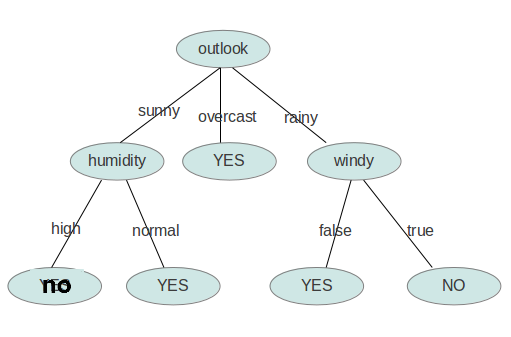
\includegraphics[width=10cm,height=7cm]{6_1}
        \caption{决策树模型}
    \end{figure}

    其实,可以将决策树看成是IF-THEN 规则的集合。决策树还表示给定特征条件下类的条件概率分布。

    \subsection{决策树的学习}

    给定一个数据集合D,每一个实例都有特征和类标签。要生成一颗决策树,使得它能对数据集合D有很好的拟合,同时还要求对未知数据可以进行预测。决策树的学习同样是最小化损失函数。损失函数是正则化的极大似然估计。

    决策树的构造如下:
    1. 开始构造根节点,将所有数据都放入根节点
    2. 选择一个最有特征,按照这一特征将训练数据分割成子集,使得各个子集在当前条件下有一个是最好的分类,如果这些子集都能被正确分类,那么构造叶节点,否则,重复步骤2。直到所有的训练数据都被正确分类,或者没有合适的特征。

    这就生成了一棵决策树。上述方法构造的决策树对训练数据集有着很好的拟合,但是对于未知数据的预测却不一定有很好的分类能力,即上述过程可能导致过拟合的问题。解决这一问题的方法是对决策树进行剪枝。另外,如果特征过多,在决策树开始建立之前就可以对特征进行选择。

    下边的内容会围绕决策树学习的一些算法展开讨论。

    \section{决策树模型的特征选择}
    \subsection{引言}
    决策树构建过程中的特征选择是非常重要的一步。特征选择是决定用哪个特征来划分特征空间,特征选择是要选出对训练数据集具有分类能力的特征,这样可以提高决策树的学习效率。如果利用某一个特征进行分类与随机分类的结果没有很大的差别,则称这个特征是没有分类能力的。这样的特征可以丢弃。常用的特征选择的准则是信息增益和信息增益比。
    
    \subsection{信息增益}
    要了解信息增益,我们要先知道熵与条件熵的定义。
    \subsubsection{熵}
    \textbf{熵是无序度的度量},在信息论和统计中,熵表示随机变量不确定性的度量。假设$X$是一个取有限值的离散型随机变量,它的概率分布如下:
    $$
    P(X=x_i)=p_i, i = 1,2,\dots,n
    $$
    则随机变量$X$的熵定义为:
    $$
    H(X) = -\sum_{i=1}^{n}p_i\log p_i
    $$ 
    $若p_i=0,定义0 \log 0 = 0$,从上式中可以看到,熵只依赖于$X$的分布,而与$X$的取值没有关系。熵越大,随机变量的不确定性就越大。故可以将$X的熵记作H(p):$
    
    $$
    H(p) = -\sum_{i=1}^{n}p_i\log p_i
    $$ 
    \subsubsection{条件熵}
    设有随机变量$(X,Y)$,其联合概率分布为:
    $$
    P(X=x_i, Y= y_j)=p_{ij}, i = 1,2, \dots, n; j = i = 1,2, \dots, m
    $$
    条件熵$H(Y|X)$表示在已知随机变量$X$的条件下随机变量$Y$的不确定性。随机变量$X$给定的条件下随机变量$Y$的条件熵$H(Y|X)$定义为$X$给定条件下$Y$的条件概率分布的熵对$X$的数学期望:
    $$
    H(Y|X)=\sum_{i=1}^{n}p_iH(Y|X=x_i), \\
    p_i=P(X=x_i), i = 1,2,\dots,n
    $$
    当熵和条件熵中的概率由数据估计得来时,所对应的熵和条件熵称为经验熵和经验条件熵。
    
    \subsubsection{信息增益}
    信息增益表示得知特征$X$的信息而使得类$Y$的信息不确定性减少的程度。
    **信息增益** 
    特征$A$对训练数据集$D$的信息增益$g(D,A)$,定义为集合$D$的经验熵$H(D)$与特征$A$给定条件下$D$的经验条件熵$H(D|A)$之差:
    $$
    g(D,A) = H(D) - H(D|A)
    $$
    信息增益大的特征具有更强的分类能力。
    根据信息增益准则进行特征选择的方法是:对训练数据集$D$,计算其每个特征的信息增益,并比较它们的大小,选择最大的特征。
    
    \subsection{信息增益比}
    
    通过信息增益选取特征的时候,存在偏向于选择取值较多的特征的问题。使用信息增益比可以纠正这一问题。
    
    \textbf{信息增益比}
    特征$A$对训练数据集$D$的信息增益比$g_R(D,A)$定义为其信息增益$g(D,A)$与训练数据集$D$关于特征$A$的值的熵$H_A(D)$之比,即:
    $$
    g_R(D,A) = \frac{g(D,A)}{H_A(D)} \\
    H_A(D) = -\sum_{i=1}^{n}\frac{|D_i|}{|D|} \log_2 \frac{|D_i|}{|D|}
    $$
    $n$是特征$A$取值的个数。

    \section{决策树的生成与剪枝}
    \subsection{决策树的生成算法}
    基本的决策树生成算法主要有ID3和C4.5, 它们生成树的过程大致相似,ID3是采用的信息增益作为特征选择的度量,而C4.5采用信息增益比。
    构建过程如下:
    \begin{enumerate}[itemindent=2em]
        \item 从根节点开始,计算所有可能的特征的信息增益(信息增益比),选择计算结果最大的特征。
        \item 根据算出的特征建立子节点,执行第一步,直到所有特征的信息增益(信息增益比)很小或者没有特征可以选择为止。
    \end{enumerate}

    以上算法只有树的生成,容易产生过拟合。

    \subsection{决策树的剪枝}
    决策树对于训练数据有很好的分类,但是对于未知测试集的分类并没有那么准确,这就产生过拟合的现象。
    其实,原理都是一样,决策树的构建是直到没有特征可选或者信息增益很小,
    这就导致构建的决策树模型过于复杂,而复杂的模型是通过在训练数据集上建立的,
    所以对于测试集往往造成分类的不准确,这就是过拟合。解决过拟合的方法是控制模型的复杂度,
    对于决策树来说就是简化模型,称为剪枝。很形象的就是减掉树中的一些节点。
    决策树的剪枝一般通过极小化损失函数或者代价函数来实现。


    设树$T$的叶节点的个数为$|T|$,$t$是树$T$的叶节点,该叶节点上有$N_t$个样本点,其中$k$类样本点有
    $N_{tk}$个,$k=1,2,\dots,K;H_t(T)$为叶节点$t$上的经验熵,$\alpha \ge 0$ 为参数,则决策树的损失函数可以定义为:
    $$C_{\alpha}(T)=\sum_{t=1}^{|T|}N_tH_t(T)+\alpha|T| (1)$$
    其中,经验熵为:
    $$H_t(T)=-\sum_k\frac{N_{tk}}{N_t} \log \frac{N_{tk}}{N_t}(2)$$
    将(1)式的第一项记为:
    $$C(T) = \sum_{t=1}^{|T|}N_tH_t(T) = -\sum_{t=1}^{|T|}\sum_{k=1}^KN_{tk} \log \frac{N_{tk}}{N_t}$$
    则:
    $$C_{\alpha}(T)=C(T)+\alpha|T| (3)$$

    $C(T)$表示模型对训练数据的预测误差,即拟合度。$|T|$表示模型的复杂度,参数$\alpha \ge 0$控制两者之间的影响。剪枝就是当$\alpha$确定时,选择损失函数最小的模型。子树越大,数据拟合得越好,但是模型的复杂度越高;相反,字数越小,数据拟合较差,模型的复杂度较低。损失函数正好表示对两者的平衡。

    从上述分析可以看出,决策树的生成算法的模型复杂度很高,很好的地拟合了训练数据。需要重点提一下的是,(3)式定义的损失函数极小化等价于正则化的极大似然估计。
    
    
    \chapter{逻辑回归}
    \section{Logistic 和 Softmax 函数}
    \subsection{说明}
    在逻辑回归和一些机器学习算法中, Logistic函数和Softmax函数是常用到的,
    今天就先讨论下这两个函数。
    \subsection{Logistic 函数}
    Logistic function一般用于二分类问题,它的函数定义如下:
    \begin{equation}
        f(x) = \frac{1}{1+e^{-x}}
    \end{equation}
    
    它的图像如下:
    \begin{figure}[h]
        \begin{center}
            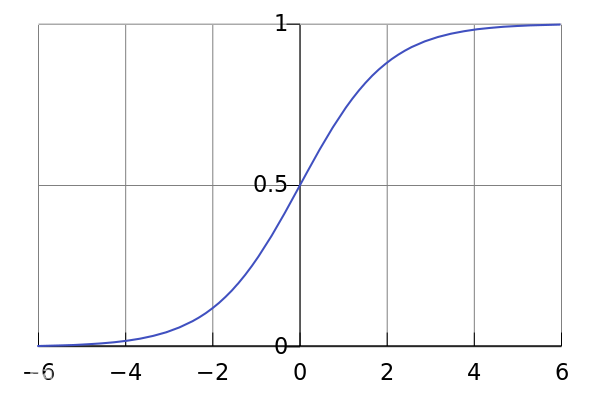
\includegraphics[width=10cm, height=8cm]{7_1.jpg}
            \caption{Logistic 函数图形}
        \end{center}
    \end{figure}
    
    由于logistic 函数的图形很像S,所以也叫sigmod 曲线。下面求一下logistic函数的导数,它在机器学习算法的推导过程中可能用到。
    \begin{equation}
        \begin{aligned}
            f'(x) &= [(1+e^{-x})^{-1}]' \\
            &= -(1+e^{-x})^{-2}*e^{-x}*(-1) \\
            &= \frac{e^{-x}}{(1+e^{-x})^2} \\
            &= \frac{1}{1+e^{-x}} \frac{e^{-x}}{1+e^{-x}} \\
            &= \frac{1}{1+e^{-x}} \frac{1+e^{-x}-1}{1+e^{-x}} \\
            &=\frac{1}{1+e^{-x}} (1- \frac{1}{1+e^{-x}}) \\
            &=f(x)[1-f(x)]
        \end{aligned}
    \end{equation}
    
    
    即 
    \begin{equation}
        f'(x)=f(x)[1-f(x)]
    \end{equation}
    
    通过logistic函数,可以把变量$x$映射到[0, 1]之间,
    在分类问题上,x是训练集上数据和对应维度特征参数的组合:
    $\boldsymbol{\theta ^Tx}+b$, 具体会在后边讲到。
    
    \subsection{Softmax 函数}
    Softmax function 是sigmod 函数的扩展,它可以用于多分类问题。它的定义如下所示:
    \begin{equation}
        Y_k =\phi(z_k)= \frac{e^{z_k}}{\sum_{i=1}^Ke^{z_i}}, k= 1,2, \dots, K
    \end{equation}

    其中,$z$往往是关于参数和样本数据的复合函数,
    softmax 函数的目的是求使得$Y_k $取值最大的$z$中的参数,$k$表示有k个分类。
    \begin{figure}[h]
        \begin{center}
            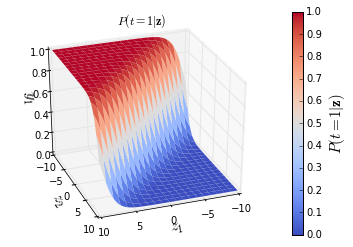
\includegraphics[width=8cm, height=5cm]{7_2.jpg}
            \caption{$Y_k$概率分布图}
        \end{center}
    \end{figure}

    图中的$P(t|z)$表示对于给定的输入$z$,它属于t的概率值。关于具体的推导,可参照文献2. 但是注意,文献2 中的$\phi_K = \frac{\phi_i}{e^{\beta_i}}$, 有问题请随时留言。
    
    \section{逻辑回归的推导过程}
    \subsection{引言}
        虽然说是逻辑回归,其实既可以用它做回归,也可以用它做分类。
        一般我们从最简单的二分类问题开始了解他,当然也可以做多分类。

    \subsection{Logistic Regression 的一般步骤}
    \begin{itemize}
        \item 找一个合适的假设
        \item 构造损失函数
        \item 让损失函数最小,求出对应的参数值
    \end{itemize}


    \subsection{二分类问题下Logistic Regression的过程}

    \subsubsection{Logistic Function}
    在上一节已经讲过了,直接给出公式:
    \begin{equation}
        f(x) = \frac{1}{1+e^{-x}}
    \end{equation}

    \subsubsection{找一个合适的假设}
    假设样本是各个贷款人的信息,标签是他是否违约。目标是建立一个模型,用来预测一个贷款人违约的可能性,而银行根据这个信息决定是否放款给当前的贷款人。那么,很明显,这是一个分类问题,根据贷款人的一些信息和已知的标签,我们建立模型,去预测新来的贷款人违约的可能性。这里将贷款人的各个信息,如学历、年收入、信用卡违约次数等作为$\boldsymbol{x}$,将他是否违约记为$y$,其中$y=1$表示违约,$y=0$表示不违约。那么,一个贷款人违约的可能性为:
    \begin{equation}
        \begin{aligned}
            h_{\boldsymbol{\theta}}(\boldsymbol{x})&=g(\boldsymbol{\theta}^T\boldsymbol{x}) \\
            &= \frac{1}{1+e^{-\boldsymbol{\theta}^T\boldsymbol{x}}}
        \end{aligned}
    \end{equation}


    其中,$\boldsymbol{\theta}$是参数向量。
    通过上式,可以将借款人的各个信息映射到(0,1)之间,
    表示他是否违约的可能性。
    \begin{equation}
        \begin{aligned}
            &P(y=1|\boldsymbol{x}; \boldsymbol{\theta}) = h_{\boldsymbol{\theta}}(\boldsymbol{x})\\
            &P(y=0|\boldsymbol{x}; \boldsymbol{\theta}) = 1 - h_{\boldsymbol{\theta}}(\boldsymbol{x})
        \end{aligned}
    \end{equation}

    将上式表示成一个式子:
    $$
    P(y|\boldsymbol{x}; \theta) = h_{\theta}(\boldsymbol{x})^y(1-h_{\theta}(\boldsymbol{x}))^{1-y}
    $$
    至此,得到了一个给定贷款人信息时,他违约概率的表达式。

    \subsubsection{构造损失函数}
    在整个样本集中,$m$个独立样本出现的似然函数是:
    $$
    L(\boldsymbol{\theta}) = \prod_{i=1}^{m}P(y_i|\boldsymbol{x_i}; \boldsymbol{\theta})
    $$
    利用最大似然求$\theta$,取对数最大似然:
    $$
    l(\boldsymbol{\theta}) = \log L(\boldsymbol{\theta}) = \sum_{i=1}^{m}\log P(y_i|\boldsymbol{x_i}; \boldsymbol{\theta})
    $$
    定义下式为损失函数:
    \begin{equation}
        \begin{aligned}
            J(\boldsymbol{\theta}) = -\frac{1}{m}l(\boldsymbol{\theta})  = -\frac{1}{m}\sum_{i=1}^{m}\log [h_{\boldsymbol{\theta}}(\boldsymbol{x_i})^{y_i}(1-h_{\boldsymbol{\theta}}(\boldsymbol{x_i}))^{1-y_i}] \\
            =-\frac{1}{m}\sum_{i=1}^{m}\{y_i \log h_{\boldsymbol{\theta}}(\boldsymbol{x_i})+(1-y_i)\log [1-h_{\boldsymbol{\theta}}(\boldsymbol{x_i})]\}
        \end{aligned}
    \end{equation}
    
    最大化$l(\theta) $相当于最小化$J(\theta)$.

    \subsubsection{让损失函数最小,求出对应的参数值}
    优化的目标函数如下:
    $$
    \min J(\boldsymbol{\theta})
    $$
    由于上式中的$\boldsymbol{\theta}$是一个参数向量,因此,没办法用函数导数等于0直接求出,它是没有解析解的,因此,我们可以采用梯度下降的方法求得极小值。梯度下降方法请参照[最优化学习笔记(三)——梯度下降法](http://blog.csdn.net/chunyun0716/article/details/51474158)。
    $$
    \frac{\partial J(\boldsymbol{\theta})}{\partial \boldsymbol{\theta}} =  -\frac{1}{m}\sum_{i=1}^{m}\{\frac{\partial T(\boldsymbol{\theta})}{\partial \boldsymbol{\theta}}\} (1)
    $$
    其中:
    \begin{equation}
        T(\boldsymbol{\theta}) = y \log h_{\boldsymbol{\theta}}(\boldsymbol{x})+(1-y)\log [1-h_{\boldsymbol{\theta}}(\boldsymbol{x})]
    \end{equation}
    
    \begin{equation}
        \begin{aligned}
            \frac{\partial T(\boldsymbol{\theta})}{\partial \boldsymbol{\theta}} &= y\frac{1}{h_{\boldsymbol{\theta}}(\boldsymbol{x})}\frac{\partial h_{\boldsymbol{\theta}}(\boldsymbol{x})}{\partial \boldsymbol{\theta}}+(1-y)\frac{1}{1-h_{\boldsymbol{\theta}}(\boldsymbol{x})}(-\frac{\partial h_{\boldsymbol{\theta}}(\boldsymbol{x})}{\partial \boldsymbol{\theta}})\\
            &=\frac{\partial h_{\boldsymbol{\theta}}(\boldsymbol{x})}{\partial \boldsymbol{\theta}}(\frac{y}{h_{\boldsymbol{\theta}}(\boldsymbol{x})}+\frac{(y-1)}{1-h_{\boldsymbol{\theta}}(\boldsymbol{x})})\\
            &=\frac{\partial h_{\boldsymbol{\theta}}(\boldsymbol{x})}{\partial \boldsymbol{\theta}}(\frac{y-{h_{\boldsymbol{\theta}}(\boldsymbol{x})}}{{h_{\boldsymbol{\theta}}(\boldsymbol{x})}(1-{h_{\boldsymbol{\theta}}(\boldsymbol{x})})})
        \end{aligned}
    \end{equation}
 
    因为:
    $$
    \frac{\partial h_{\boldsymbol{\theta}}(\boldsymbol{x})}{\partial \boldsymbol{\theta}} = {h_{\boldsymbol{\theta}}(\boldsymbol{x})}(1-{h_{\boldsymbol{\theta}}(\boldsymbol{x})})\boldsymbol{x}
    $$

    则:
    $$
    T(\boldsymbol{\theta}) = (y-{h_{\boldsymbol{\theta}}(\boldsymbol{x})})\boldsymbol{x}
    $$
    由于取的是样本集中的第$i$ 个样本,所以将上式代入(1)
    \begin{equation}
        \begin{aligned}
            \frac{\partial J(\boldsymbol{\theta})}{\partial \boldsymbol{\theta}} &=  -\frac{1}{m}\sum_{i=1}^{m} (y_i-{h_{\boldsymbol{\theta}}(\boldsymbol{x_i})})\boldsymbol{x_i}\\
            &=\frac{1}{m}\sum_{i=1}^{m} ({h_{\boldsymbol{\theta}}(\boldsymbol{x_i})}-y_i)\boldsymbol{x_i}
        \end{aligned}
    \end{equation}
    
    这样,就可以得到$\boldsymbol{\theta}$的迭代公式:
    \begin{equation}
        \begin{aligned}
            \boldsymbol{\theta} &= \boldsymbol{\theta} + \alpha\frac{\partial J(\boldsymbol{\theta})}{\partial \boldsymbol{\theta}} \\
            &=\boldsymbol{\theta} + \alpha\frac{1}{m}\sum_{i=1}^{m} ({h_{\boldsymbol{\theta}}(\boldsymbol{x_i})}-y_i)\boldsymbol{x_i}
    \end{aligned}
    \end{equation}
   
    需要说明的是,我们可以从2式中看出,每次计算一次$\boldsymbol{\theta} $,都要进行全部样本数据的计算,直到$\boldsymbol{\theta} $收敛,还有一种可以采用随机梯度法进行计算,这样只需要遍历一遍数据集即可,下次讨论。

    \chapter{隐马尔科夫模型}

    \section{简介}
    在马尔科夫模型中,每一个状态代表了一个可以观察的事件,所以,马尔科夫模型有时称为可视马尔科夫模型(visible Markov model,VMM),
    这在某种程度上限制了模型的适应性。在隐马尔科夫模型(HMM)中,我们不知道模型所经过的状态序列,而只知道状态的概率函数,也就是说观察到的事件是状态的随机函数,此模型是一个双重的随机过程。其中,模型的状态转换过程是隐蔽的,可观察事件的随机过程是隐蔽的状态转换过程的随机函数。
    
    \section{隐马尔科夫模型的基本原理}
    下图是一个隐马尔科夫模型的示意图,用此图来说明HMM的原理。
    假设一个暗室中有$N$个口袋,每个口袋中有$M$种不同颜色的球。
    一个实验员根据某一概率分布随机选取一个初始的口袋,从中根据不同颜色球的概率分布,
    随机选取出一个球,并向室外的人报告该球的颜色。然后再根据口袋的概率分布选择另一个口袋,根据不同颜色球的概率分布随机选择一个球,重复进行这个过程。对于室外的观察人员来说,他只能观察到不同颜色球的序列,口袋的序列不可观察。在这个过程中,口袋对应HMM中的状态,球的颜色对应HMM中状态的输出,从一个口袋到另一个口袋对应于状态的转换,从口袋中取出球的颜色对应于从一个状态输出的观察符号。

    \begin{figure}[h]
        \begin{center}
            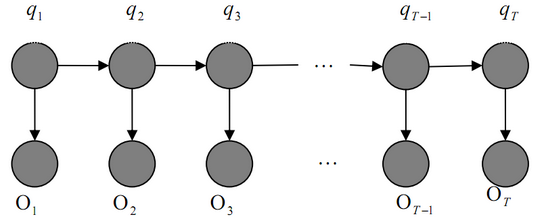
\includegraphics[width=13cm, height=5.5cm]{8_1.jpg}
            \caption{马尔科夫状态图}
        \end{center}
    \end{figure}

    \subsection{HMM的组成部分}
    \begin{enumerate}
        \item 模型中状态的数目$N$(口袋的数目)
        \item 从每个状态可能输出的不同符号的数目$M$(球的不同颜色的数目)
        \item 状态转移概率矩阵$\boldsymbol{A} = \{a_{ij}\}$,其中
        \begin{equation}
            \begin{split}
                &a_{ij}=P(q_t=s_j|q_{t-1},s_i)\\
                &1 \le i, \\
                &j \le N,  \\
                &a_{ij} \ge 0, \\
                &\sum_{j=1}^N a_{ij} = 1
            \end{split}
        \end{equation}
        
        
        \item 从状态$S_j$观察到符号$v_k$的概率分布$\boldsymbol{B} = \{b_j(k)\}$,其中
        \begin{equation}
            \begin{split}
                &b_j(k) = P(O_t = v_k|q_t=s_j),\\
                &1 \le j \le N, \\
                &1\le k \le M,\\
                &b_j(k) \ge 0,\\
                &\sum_{k=1}^M b_j(k)  = 1
            \end{split}
        \end{equation}
        
        观察符号的概率又称为发射概率
        \item 初始状态的概率分布$\boldsymbol{\pi} = \{\pi_i\}$,其中
        \begin{equation}
            \begin{split}
                &\pi_i=P(q_1=s_i), \\
                &1 \le i \le N ,\\
                &\pi_i \ge 0, \\
                &\sum_{i=1}^N \pi_i= 1
            \end{split}
        \end{equation}
    \end{enumerate}

    一般地,一个HMM记为一个五元组$ \mu =(S,K,\boldsymbol{A},\boldsymbol{B},\boldsymbol{\pi})$,其中,$S$为状态集合,$K$为输出符号的集合,$\boldsymbol{A}$为状态转移矩阵,$\boldsymbol{B}$为符号的发射概率,$\boldsymbol{\pi}$为初始状态的概率分布。有时也记为$ \mu =(\boldsymbol{A},\boldsymbol{B},\boldsymbol{\pi})$

    \subsection{观察序列的生成}
    当考虑潜在事件随机地生成表面事件时,HMM非常有用。
    假设给定模型$ \mu =(\boldsymbol{A},\boldsymbol{B},\boldsymbol{\pi})$,
    那么观察序列$O=O_1O_2\dots O_T$可由下面的步骤产生:
    \begin{enumerate}
        \item 根据初始的状态概率分布$\pi_i$选择一个初始的状态$q_1=s_i$
        \item 设t=1
        \item 根据状态$s_i$的输出概率分布$b_i(k)$输出$O_t=v_k$
        \item 根据状态转移概率分布$a_{ij}$,将当前$t$时刻的状态转移到新的状态$q_{t+1}=s_j$
        \item $t = t+1$, 如果$t<T$,重复执行步骤3,4.否则,算法结束。
    \end{enumerate}

    \section{HMM估计问题和前向后向算法}

    \subsection{隐马尔科夫链的第一个基本问题}
    估计问题:给定一个观察序列$O=O_1O_2\dots O_T$和
    模型$u = (\boldsymbol{A,B,\pi})$,如何快速地计算出给定模型$u$情况下,
    观察序列$O$的概率, 即$P(O|u)$?

    \subsection{求解观察序列的概率}
    其实,求解这个问题就是一个解码问题。
    对于任意的状态序列$Q=q_1q_2\dots q_T$,有
    \begin{equation}
        \begin{split}
            P(O|Q,u)&= \prod_{t=1}^{T-1} P(O_t|q_t,q_t+1,u) \\
            &=b_{q1}(O_1)b_{q2}(O_2)\dots b_{qT}(O_T)
        \end{split}
    \end{equation}
    
    并且
    \begin{equation}
        P(Q|u) = \pi _{q_1}a_{q_1q_2}a_{q_2q_3} \dots a_{q_{T-1}q_T}
    \end{equation}
    由于
    \begin{equation}
        P(O,Q|u) = P(O|Q,u)P(Q|u)
    \end{equation}
    所以
    \begin{equation}
        \begin{split}
            P(O|u) &= \sum _{Q} P(O,Q|u) \\
            &=\sum _{Q}P(O|Q,u)P(Q|u) \\
            &=\sum _{Q}\pi _{q_1}b_{q1}(O_1)\prod_{t=1}^{T-1}a_{q_{t}q_{t+1}}b_{q_{t+1}}(O_{t+1})
        \end{split}
    \end{equation}
    上述推导过程很直接,但是实际的计算量是非常庞大的,
    它要穷尽所有可能的状态序列,如果模型中有$N$个状态,时间长度为$T$,
    那么有$N^T$个可能的状态序列,这导致了并不能有效地执行这个算法。
    因此,人们提出了前向算法,利用动态规划来解决指数爆炸的问题。

    \subsection{HMM中的前向算法}

    为了实现前向算法,需要定义一个前向变量$\alpha_t(i)$.

    
    \begin{definition}
        前向变量$\alpha_t(i)$是在时间$t$, HMM输出序列$O=O_1O_2\dots O_t$并且位于状态$s_i$的概率:
        \begin{equation}
            \alpha_t(i) = P(O_1O_2\dots O_t, q_t=s_i|u)
        \end{equation}
    \end{definition} 
    

    前向算法的主要思想是,如果可以快速地计算前向变量$\alpha_t(i)$,那么就可以根据$\alpha_t(i)$计算出$P(O|u) $, 因为$P(O|u) $是在所有状态下观察到序列$O=O_1O_2\dots O_t$的概率:
    \begin{equation}
        P(O|u) = \sum _{s_i}P(O_1O_2\dots O_T, q_T=s_i|u)= \sum _{i=1}^{N}\alpha_T(i)
    \end{equation}


    在前向算法中,采用动态规划的方法计算前向变量$\alpha_t(i)$,
    其思想基于如下观察:在时间t+1的前向变量可以根据时间t时的前向变量$\alpha_t(1),\alpha_t(2),\dots, \alpha_t(N)$来归纳计算:
    \begin{equation}
        \alpha_{t+1}(j) = (\sum_{i=1}^{N}\alpha_t(i)a_{ij})b_j({O_{t+1}}) 
    \end{equation}

    \subsubsection{前向算法}

    \begin{enumerate}
        \item 初始化: $\alpha_1(i)=\pi_ib_i(O_1), 1 \le i \le N$
        \item 归纳计算: $\alpha_{t+1}(j) = (\sum_{i=1}^{N}\alpha_t(i)a_{ij})b_j({O_{t+1}}) , 1 \le t \le T-1$
        \item 求和终结: $P(O|u) = \sum _{i=1}^{N}\alpha_T(i)$
    \end{enumerate}

    前向算法的时间复杂度为$O(N^2T)$

    \subsection{HMM中的后向算法}
    快速计算$P(O|u)$还有一种后向算法。
    对应于前向变量,定义一个后向变量$\beta_t(i)$.
    \begin{definition}
        后向变量$\beta_t(i)$是在给定模型$u = (\boldsymbol{A,B,\pi})$并且在时间$t$状态为$s_i$的条件下,HMM的输出观察序列$O=O_{t+1}O_{t+2}\dots O_T$的概率:
        \begin{equation}
            \beta_t(i) = P(O_{t+1}O_{t+2}\dots O_T| q_t=s_i|u)
        \end{equation}
    \end{definition} 
    
    类似于前向算法,也可以用动态规划算法计算后向变量。
    \begin{enumerate}
        \item 从时间$t$到时间$t+1$, HMM的状态$s_i$到状态$s_j$输出$O_{t+1}$,概率为$a_{ij}b_j(O_{t+1})$
        \item 在时间$t+1$的状态为$s_j$的条件下,HMM输出观察序列$O_{t+2}\dots O_T$,概率为:$\beta_{t+1}(j) $
        则,归纳关系为:
        \begin{equation}
            \beta_t(i)=\sum_{j=1}^{N}a_{ij}b_j(O_{t+1})\beta_{t+1}(j)
        \end{equation}
    \end{enumerate}
   

    \subsection{后向算法}
    \begin{enumerate}
        \item 初始化:$\beta_T(i)=1, 1 \le i \le N$
        \item 归纳计算:$\beta_t(i)=\sum_{j=1}^{N}a_{ij}b_j(O_{t+1})\beta_{t+1}(j), T-1 \ge t \ge 1; 1 \le i \le N$
        \item 求和终结:$P(O|u) = \sum _{i=1}^{N}\pi_ib_i(O_1)\beta_1(i)$
    \end{enumerate}

    后向算法的时间复杂度为$O(N^2T)$

    \section{HMM序列问题和维特比算法}
    \subsection{HMM中的第二个基本问题}
    序列问题:给定一个观察序列$O=O_1O_2\dots O_T$和
    模型$u=(\boldsymbol{A,B,\pi})$,
    如何快速有效地选择在一定意义下"最优"的状态序列
    $Q=q_1q_2\dots q_T$,使得该状态序列“最好地解释”观察序列?

    \subsection{定义最优状态序列}
    序列问题的答案并不是唯一的,那是因为它取决于对“最优状态序列的理解”。
    \textbf{最优状态序列}
    \begin{definition}
        在给定模型$u$和观察序列$O$的条件下,使得条件概率$P(Q|O,u)$最大的状态序列:
        \begin{equation}
            \hat{Q}=arg \max_Q P(Q|O,u)
        \end{equation}
    \end{definition}

    \subsection{维特比算法}
    维特比算法运用动态规划的搜索算法求解这种最优状态序列。
    为了实现这种搜索,首先定义一个维特比变量$\delta_t(i)$。
    \begin{definition}
        维特比变量$\delta_t(i)$ 是在时间$t$时,
        HMM沿着某一条路径到达状态$s_i$,
        并输出观察序列$O_1O_2\dots O_t$的最大概率:
        \begin{equation}
            \delta_t(i) = \max_{q_1,q_2, \dots, q_t-1} P(q_1,q_2, \dots, q_t=s_i, O_1O_2\dots O_t|u)
        \end{equation}
    \end{definition}
    与前向变量类似,$\delta_t(i)$有如下递推关系:
    \begin{equation}
        \delta_{t+1}(i) =  \max_j[\delta_t(j)a_{ji}]b_i(O_{t+1})
    \end{equation}


    为了记录在时间$t$时,HMM通过哪一条概率最大的路径到达状态$s_i$,
    维特比算法设置了另外一个变量$\psi_t(i)$,用于路径记忆,
    让$\psi_t(i)$记录该路径上的状态$s_i$的前一个(在时间$t-1$)状态。

    \subsubsection{维特比算法}
    \begin{enumerate}
        \item 初始化
        \begin{equation}
            \begin{split}
                \delta_1(i) = \pi_ib_i(O_1), 1 \le i \le N \\
                \psi_1(i) = 0
            \end{split}
        \end{equation}
        \item 归纳计算
        \begin{equation}
            \begin{split}
                &\delta_{t}(j) =  \max_{1 \le i \le N}[\delta_{t-1}(i)a_{ij}]b_j(O_t), 2 \le t \le T; 1 \le j \le N\\
                &\psi_t(j) =arg  \max_{1 \le i \le N}[\delta_{t-1}(i)a_{ij}]b_j(O_t), 2 \le t \le T; 1 \le i \le N\\
            \end{split}
        \end{equation}
        \item 终结
        \begin{equation}
            \begin{split}
                &\hat{Q_T} = arg \max_{1 \le i \le N}[\delta_{T}(i)]\\
                &\hat{P}(\hat{Q_T}) = \max_{1 \le i \le N}[\delta_{T}(i)]\\
            \end{split}
        \end{equation}
        \item 路径(状态序列)回溯
            \begin{equation}
                \hat{q_t} = \psi_{t+1}(\hat{q}_{t+1} ) , t =T-1, T-2, \dots, 1
            \end{equation}
    \end{enumerate}

        维特比算法的时间复杂度也是$O(N^2T)$。

    \section{HMM的参数估计}
    \subsection{HMM中的第三个基本问题}
    参数估计问题:给定一个观察序列$O=O_1O_2\dots O_T$,
    如何调节模型$\mu = (A, B, \pi)$的参数,使得$P(O|\mu)$最大化:
    \begin{equation}
        arg \max_{\mu} P(O_{training}|\mu)
    \end{equation}

    模型的参数是指构成$\mu$的$\pi_i,a_{ij}, b_j(k)$。
    本文的前序两节讲的EM算法就是为了解决模型参数的最大化问题。
    其基本思想是,初始时随机地给模型参数赋值,该赋值遵循模型对参数的限制,
    例如,从某一状态出发的所有转移概率之和为1.给模型参数赋初值后,
    得到模型$\mu_0$, 然后根据$\mu_0$可以得到模型中隐变量的期望值。
    例如,从$\mu_0$得到某一状态到另一状态的期望次数,
    用期望次数来替代实际次数,这样可以得到模型参数的重新估计值,
    由此得到新的模型$\mu_1$。然后重复上述过程,直到参数收敛于最大似然估计值。

    \subsection{算法介绍}
    给定HMM的参数$\mu$和观察序列$O=O_1O_2\dots O_T$在时间$t$位于状态$s_i$,
    时间$t+1$位于状态$s_j$的概率:
    \begin{equation}
        \xi_t(i,j) = P(q_t=s_i, q_{t+1} = s_j | O; \mu)(1 \le t \le T, 1 \le i,j \le N)
    \end{equation}

    可由下面的公式计算获得:
    \begin{equation}
        \begin{split}
            \xi_t(i,j) &= \frac{P(q_t=s_i, q_{t+1} = s_j , O; \mu)}{P(O;\mu)} \\
            &=\frac{a_t(i)a_{ij}b_j(O_{t+1})\beta_{t+1}(j)}{P(O;\mu)}\\
            &=\frac{a_t(i)a_{ij}b_j(O_{t+1})\beta_{t+1}(j)}{\sum_{i=1}^N\sum_{j=1}^Na_t(i)a_{ij}b_j(O_{t+1})\beta_{t+1}(j)}(18-1)
        \end{split}
    \end{equation}

    给定HMM的参数$\mu$和观察序列$O=O_1O_2\dots O_T$
    在时间$t$位于状态$s_i$的概率$\gamma_t(i)$为:
    \begin{equation}
        \gamma_t(i) = \sum_{j=1}^N \xi_t(i,j)
    \end{equation}
 
    由此,$\mu$的参数可由下式估计:
    \begin{equation}
        \begin{split}
            &\bar{\pi_i} = P(q_1=s_i |O; \mu) = \gamma_1(i)\\
            &\bar{a}_{ij}= \frac{Q\mbox{中从状态}q_i\mbox{转移到}q_j\mbox{的期望次数}}{Q\mbox{中所有从状态}q_i\mbox{转移到另一状态(包含}q_j\mbox{)的期望次数}}=\frac{\sum_{t=1}^{T-1}\xi_t(i,j) }{\sum_{t=1}^{T-1}\gamma_t(i)}\\
            &\bar{b}_j(k) = \frac{Q\mbox{中从状态}q_j\mbox{输出符号}v_k\mbox{的期望次数}}{Q\mbox{到达}q_j\mbox{的期望次数}}=\frac{\sum_{t=1}^{T}\gamma_t(j)\delta(O_t, v_k)}{\sum_{t=1}^{T}\gamma_t(j)}
        \end{split}
    \end{equation}


    \subsection{前向后向算法}
    根据上述思路,给出前向后向算法:
    \begin{enumerate}
        \item 初始化:随机地给参数$\pi_i,a_{ij}, b_j(k)$赋值,使得满足如下约束:
        \begin{equation}
            \begin{split}
                \sum_{i=1}^N \pi_i=1\\
                \sum_{j=1}^N a_{ij} =1, 1 \le i \le N\\
                \sum_{k=1}^M b_j(k) =1, 1 \le j \le N
            \end{split}
        \end{equation}
        由此,得到模型$\mu_0$.令$i=0$,执行下面的EM估计。
        \item EM计算
        E步:由模型$\mu_i$根据公式18-1和18-2计算$\xi_t(i,j)$和$\gamma_t(i)$;
        M步:用E步得到的期望值重新估计模型参数$\pi_i,a_{ij}, b_j(k)$,得到模型$\mu_{i+1}$
        \item 循环计算:
        令 $i = i+1$, 重复EM计算,直到$\pi_i,a_{ij}, b_j(k)$收敛。
    \end{enumerate}

    \chapter{EM算法}
    \section{EM简介}

    \subsection{引言}
    按照计划,这周应该学习HMM中的第三个基本问题:参数估计问题,但是其中的内容涉及到了EM算法,所以打算先把EM算法搞定之后再去继续HMM的问题。EM算法的推导过程比较复杂,
    这节我只给出简述和计算公式,待推导完成后再贴上推导过程。

    \subsection{一个实例}
    \textbf{例1 (三硬币模型)}假设有3枚硬币,分别记为$A,B,C$。
    这些硬币正面出现的概率分别是$\pi, p,q$。进行如下掷硬币试验:
    先掷硬币A,根据其结果选出B或者C,正面选B,反面选C;然后掷选出的硬币,
    掷硬币的结果,正面记为1,反面记为0;独立重复n次试验(这里,n=10),观测结果如下:1,1,0,1,0,0,1,0,1,1.假设只能观测到掷硬币的结果,不能观测掷硬币的过程。
    问如何估计三硬币正面出现的概率,即求三硬币模型的参数。

    三硬币模型可以写作:
    \begin{equation}
        \begin{split}
            P(y;\theta) &= \sum_z P(y,z;\theta)\\ 
            &= \sum_z P(z;\theta)P(y|z;\theta) \\
            &=\pi p^y(1-p)^{1-y}+(1-\pi)q^y(1-q)^{1-y}
        \end{split}
    \end{equation}

    上式中,随机变量$y$是观测变量,$z$是隐变量且不可观测,
    $\theta = (\pi, p, q)$是模型参数。这一模型是以上数据的生成模型。
    将观测数据表示为$Y=(Y_1,Y_2,\dots,Y_n)^T$, 
    未观测数据表示为$Z=(Z_1,Z_2, \dots, Z_n)^T$,则观测数据的似然函数为:
    \begin{equation}
        \begin{split}
            P(Y;\theta) &=  \sum_z P(Z;\theta)P(Y|Z;\theta) \\
            &=\prod_{j=1}^n[\pi p^{y_j}(1-p)^{1-{y_j}}+(1-\pi)q^{y_j}(1-q)^{1-{y_j}}]
        \end{split}
    \end{equation}

    \subsection{EM算法的迭代公式}
    考虑求模型参数$\theta = (\pi, p, q)$的极大似然估计,即:
    \begin{equation}
        \hat{\theta} = arg \max_\theta \log P(Y;\theta)
    \end{equation}


    这个问题没有解析解,只有通过迭代方法求解,
    EM算法就是求解这个问题的一种算法。下面先给出去针对上述问题的EM算法,
    推导过程下节给出。
    \begin{enumerate}
        \item 选取初始参数 
        \begin{equation}
            \theta^{(0)} = (\pi^{(0)}, p^{(0)}, q^{(0)})
        \end{equation}
        \item E步:计算模型参数
        \begin{equation}
            \pi^{(i)}, p^{(i)}, q^{(i)}
        \end{equation}
        下观测数据$y_j$来自掷硬币B的概率:
        \begin{equation}
            \mu^{(i+1)} = \frac{\pi^{(i)}(p^{(i)})^{y_j}(1-p^{(i)})^{1-y_j}}{\pi^{(i)}(p^{(i)})^{y_j}(1-p^{(i)})^{1-y_j} +(1-\pi^{(i)})(q^{(i)})^{y_j}(1-q^{(i)})^{1-y_j}}
        \end{equation}
        \item M步:计算模型参数的新估计值:
        \begin{equation}
            \pi^{(i+1)} = \frac{1}{n}\sum_{j=1}^{n}\mu_j^{(i+1)}
        \end{equation}
        \begin{equation}
            p^{(i+1)} = \frac{\sum_{j=1}^{n}\mu_j^{(i+1)}y_j}{\sum_{j=1}^{n}\mu_j^{(i+1)}}
        \end{equation}
        \begin{equation}
            q^{(i+1)} = \frac{\sum_{j=1}^{n}(1-\mu_j^{(i+1)})y_j}{\sum_{j=1}^{n}(1-\mu_j^{(i+1)})}
        \end{equation}
        \item 给出停止迭代的条件, 一般是较小的正数$\varepsilon$, 满足:
        \begin{equation}
            ||\theta^{(i+1)}-\theta^{(i)}|| < \varepsilon
        \end{equation}
    \end{enumerate}
    重复上式2-4步,完成求解,需要注意的是EM算法对初始值的选取是相当敏感的。

    \section{EM算法的推导}
    \subsection{Jensen 不等式}
    在EM算法的推导过程中,用到了数学上的Jensen不等式,这里先来介绍一下。
    若Ω是有限集合$\{x_1,x_2,\ldots,x_n\}$,而μ是Ω上的正规计数测度,
    则不等式的一般形式可以简单地用和式表示:
    \begin{equation}
        \varphi\left(\sum_{i=1}^{n} g(x_i)\lambda_i \right) \le \sum_{i=1}^{n} \varphi(g(x_i))\lambda_i
    \end{equation}

  其中$\lambda_1 + \lambda_2 + \cdots + \lambda_n = 1, \lambda_i \ge 0$。

  若$\varphi$是凹函数,只需把不等式符号调转。
  
    \subsection{EM算法推导}
    面对一个含有隐含变量的概率模型,
    目标是极大化观测数据$Y$关于参数$\theta$的对数似然函数,即极大化:
    \begin{equation}
        \begin{split}
            L(\theta) &= log P(Y;\theta) = log \sum_{z} P(Y,Z; \theta)\\
            &= log \sum_{z} P(Y|Z; \theta) P(Z; \theta)
        \end{split}
    \end{equation}


    事实上,EM算法是通过迭代逐步极大化$L(\theta)$的。假设在第$i
    $次迭代后$\theta$的估计值是$\theta^{(i)}$。
    我们希望新的估计值$\theta$能使$L(\theta)$增加,
    即$L(\theta) > L(\theta^{(i)})$,并逐步达到极大值。为此考虑两者的差:
    \begin{equation}
        \begin{split}
            L(\theta) - L(\theta^{(i)}) &=log (\sum_{z} P(Y|Z; \theta) P(Z; \theta)) - log P(Y;\theta^{(i)}) \\
            &= log (\sum_{z} P(Z|Y;\theta^{(i)}) \frac{P(Y|Z; \theta) P(Z; \theta)}{P(Z|Y; \theta^{(i)})}) - log P(Y;\theta^{(i)}) \\
            &\ge \sum_{z} P(Z|Y;\theta^{(i)}) log \frac{P(Y|Z; \theta) P(Z; \theta)}{P(Z|Y; \theta^{(i)})} -log P(Y;\theta^{(i)}) \\
            &= \sum_{z} P(Z|Y;\theta^{(i)}) log \frac{P(Y|Z; \theta) P(Z; \theta)}{P(Z|Y; \theta^{(i)})P(Y;\theta^{(i)})}
        \end{split}
    \end{equation}

    上式利用了Jensen不等式, 
    令 $\varphi$ 为 $log$, 且$\sum_{z} P(Z|Y;\theta^{(i)}) =1$,
    则可得上述推导。注意\textbf{$log$为凹函数,不等号要改变方向}。

    令
    \begin{equation}
        B(\theta,\theta^{(i)}) = L(\theta^{(i)}) + \sum_{z} P(Y|Z;\theta^{(i)}) log \frac{P(Y|Z; \theta) P(Z; \theta)}{P(Y|Z; \theta^{(i)})P(Y;\theta^{(i)})}
    \end{equation}

    则:
    \begin{equation}
        L(\theta) \ge B(\theta,\theta^{(i)})
    \end{equation}

    那么,$B(\theta,\theta^{(i)})$是$L(\theta)$的一个下界:
    \begin{equation}
        L(\theta^{(i)}) = B(\theta^{(i)},\theta^{(i)})
    \end{equation}

    因此,任何可以使$B(\theta,\theta^{(i)})$增大的$\theta$,
    都可使$L(\theta)$增大,选择$\theta^{(i+1)}$
    \mbox{使}$B(\theta,\theta^{(i)})$达到极大,即:
    \begin{equation}
        \theta^{(i+1)} = arg \max_{\theta} B(\theta,\theta^{(i)})
    \end{equation}

    现在求$\theta^{(i+1)}$ 的表达式,省去对于$\theta$而言都是常数的项:
    \begin{equation}
        \begin{split}
            \theta^{(i+1)} &= arg\max_{\theta} \left(L(\theta^{(i)})+\sum_{z}P(Y|Z;\theta^{(i)}) log \frac{P(Y|Z; \theta) P(Z; \theta)}{P(Y|Z;\theta^{(i)})P(Y;\theta^{(i)})}\right)\\
            &= arg\max_{\theta} \left(\sum_{z}P(Y|Z;\theta^{(i)}) log{P(Y|Z; \theta) P(Z; \theta)}\right)\\
            &= arg\max_{\theta} \left(\sum_{z}P(Y|Z;\theta^{(i)})log P(Y,Z;\theta)\right)\\
            &= arg\max_{\theta} Q(\theta, \theta^{(i)})
        \end{split}
    \end{equation}
    EM算法并不能保证全局最优值,直观解释如图所示:
    \begin{figure}[h]
        \begin{center}
            \caption{EM优化示意图}
            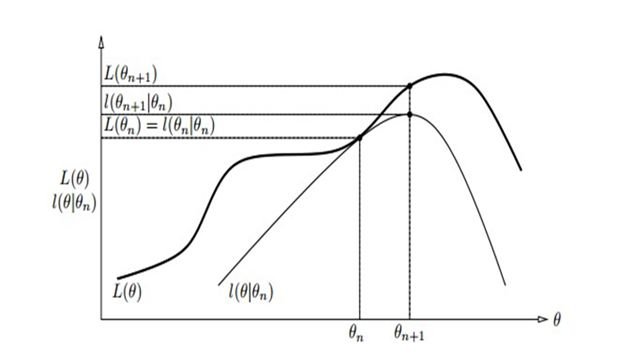
\includegraphics[width=10cm, height=8cm]{9_1.jpg}
        \end{center}
    \end{figure}

    \chapter{最大熵}

    \section{最大熵原理}
    最大熵原理是概率模型学习的一个准则。
    最大熵原理认为,在学习概率模型时,在所有可能的概率分布中,
    熵最大的模型是最好的模型。通常用约束条件来确定概率模型的集合,
    所以,最大熵模型也可以表述为在满足约束条件的模型集合中选取熵最大的模型。
    假设离散型随机变量$X$的概率分布式$P(X)$,则其熵是:
    \begin{equation}
        H(P)=-\sum_x P(x) \log P(x)
    \end{equation}


    熵满足下列不等式:
    \begin{equation}
        0 \le H(P) \le \log|x|
    \end{equation}

    式中,$|X|$是$X$取值个数,当且仅当$X$的分布是均匀分布时右边的等号成立。这就是说,当$X$服从均匀分布时,熵最大。

    \section{最大熵模型的定义}

    假设分类模型是一个条件概率分布$P(Y|X)$,
    $X \in \mathcal{X} \subseteq \mathbb{R}^n$, 
    表示输入, $Y \in \mathcal{Y}$表示输出,
    $\mathcal{X},\mathcal{Y}$分别是输入和输出的集合。
    这个模型表示的是对于给定的输入$X$,以条件概率$P(Y|X)$输出$Y$.
    给定一个训练数据集
    \begin{equation}
        T = \{(x_1, y_1),(x_2, y_2),\dots,(x_N, y_N)\}
    \end{equation}

    学习的目标是用最大熵原理选择最好的分类模型。
    对于给定的数据集,我们可以确定联合分布的经验分布和边缘分布的经验分布。
    用特征函数$f(x,y)$描述$x,y$之间的一个事实,即:
    $$
    f(x, y) = \left\{ \begin{array}{ll}
    1, & x与y满足某一事实 \\
    0, &否则
    \end{array} \right. 
    $$

    特征函数$f(x,y)$关于经验分布$\widetilde{P}(X,Y)$的期望值, 
    用$E_{\bar{p}}(f)$表示。
    \begin{equation}
        E_{\bar{p}}(f) = \sum_{x, y} \widetilde{P}(x,y) f(x,y)
    \end{equation}


    特征函数$f(x,y)$关于模型$P(Y|X)$与经验分布 $\widetilde{P}(X)$的期望值, 
    用$E_{p}(f)$表示
    \begin{equation}
        E_{p}(f) =  \sum_{x, y} \widetilde{P}(x)\widetilde{P}(y|x) f(x,y)
    \end{equation}


    如果模型可以获得训练数据中的信息, 我们就可以假设这两个期望相等:
    \begin{equation}
        E_{\bar{p}}(f) = E_{p}(f)
    \end{equation}

    \begin{definition}
        \textbf{最大熵模型}假设满足所有约束条件的模型集合为:
        \begin{equation}
            \mathcal{C} \equiv \{P \in \mathcal{P} |E_{\bar{p}}(f_i) = E_{p}(f_i), i = 1, 2 \dots, n\}
        \end{equation}
        定义在条件概率分布$P(Y|X)$上的条件熵为:
        \begin{equation}
            H(P) = -\sum_{x, y} \widetilde{P}(x) P(y|x) \log P(y|x)
        \end{equation}
        则模型集合$\mathcal{C}$中条件熵$H(P)$最大的模型称为最大熵模型,
        对数为自然对数。
    \end{definition}

    \section{求解最大熵模型}
    \subsection{问题的引出}
    最大熵模型的学习过程就是求解最大熵模型的过程。
    最大熵模型的学习可以形式化为约束最优化问题。

    对于给定的训练数据集$T=\{(x_1,y_1),(x_2,y_2),\dots,(x_n,y_n)\}$
    及特征函数$f_i(x,y), i=1, 2, \dots, n$,
    最大熵模型的学习等价于约束最优化问题:
    \begin{equation}
        \begin{split}
            &\max_{P \in C} H(P)=-\sum_{x,y} \widetilde{P}(x)P(y|x) \log P(y|x)\\
            s.t. &\quad E_p(f_i)=E_{\widetilde{p}}(f_i), i=1, 2, \dots, n \\
            &\sum_yP(y|x)=1
        \end{split}
    \end{equation}


    上式等价于:
    \begin{equation}
        \begin{split}
            &\min_{P \in C} -H(P)=\sum_{x,y} \widetilde{P}(x)P(y|x) \log P(y|x)\\
            s.t. &\quad E_p(f_i)-E_{\widetilde{p}}(f_i)=0, \quad  i=1, 2, \dots, n\\
            &\sum_yP(y|x)=1
        \end{split}
    \end{equation}


    求解上式有约束的最优化问题,所得出的解,就是最大熵模型学习的解。

    \subsection{推导过程}
    将约束最优化的原问题转换为无约束最优化问题的对偶问题,通过求解对偶问题求解原问题。
    首先,引入拉格朗日乘子$w_0, w_1, \dots, w_n$, 定义拉格朗日函数$L(P,w)$:
    \begin{equation}
        \begin{split}
            L(P,w) &= -H(P) + w_0(1-\sum_yP(y|x)) + \sum_i^n w_i(E_p(f_i)-E_{\widetilde{p}}(f_i)) \\
            &=\sum_{x,y} \widetilde{P}(x)P(y|x) \log P(y|x) + w_0(1-\sum_yP(y|x)) \\
            &+ \sum_i^n w_i(\sum_{x, y} \widetilde{P}(x,y)f_i(x,y)-\sum_{x, y} \widetilde{P}(x)P(y|x)f_i(x,y))
        \end{split}
    \end{equation}

    最优化的原始问题是:
    \begin{equation}
        \min_{P \in C} \max_w L(P,w)
    \end{equation}
    对偶问题是:
    \begin{equation}
        \max_w \min_{P \in C} L(P,w)
    \end{equation}


    由于拉格朗日函数$L(P,w)$ 是$P$的凸函数, 原问题的解与对偶问题的解是等价的。
    首先求$\min_{P \in C} L(P,w)$,  $\min_{P \in C} L(P,w)$是$w$的函数,记为:
    \begin{equation}
        \Psi(w) = \min_{P \in C} L(P_w,w),
    \end{equation}
    $\Psi(w)$的解 记为:
    \begin{equation}
        P_w = arg  \min_{P \in C} L(P,w) = P_w(y|x)
    \end{equation}
    求$L(P,w)$对$P(y|x)$的偏导数:
    \begin{equation}
        \frac{\partial{L(P,w)}}{\partial{P(y|x)}} = \sum_{x,y} \widetilde{P}(x)(\log P(y|x) + 1)- \sum_y w_0 - \sum_{x,y}(\widetilde{P}(x) \sum_{i=1}^n w_i f_i(x,y))
    \end{equation}
    令 偏导数=0 ,当$\widetilde{P}(x) > 0$时, 
    \begin{equation}
        \begin{split}
            P(y|x) &= \exp(\sum_{i=1}^n w_i f_i(x,y) + w_0 - 1) \\
            &= \frac{\exp(\sum_{i=1}^n w_i f_i(x,y))}{\exp(1- w_0)}
        \end{split}
    \end{equation}

    由于$\sum_yP(y|x)=1$得:
    \begin{equation}
        \exp(1- w_0) = \sum_y \exp(\sum_{i=1}^n w_i f_i(x,y)) = Z_w(x) 
    \end{equation}

    \begin{equation}
        P_w(y|x) = \frac{1}{Z_w(x)}\exp(\sum_{i=1}^n w_i f_i(x,y))
    \end{equation}

    其中, $Z_w(x)$称为规范化因子, $f_i(x,y)$为特征函数, $w_i$是特征权值。
    $P_w(y|x)$就是最大熵模型。之后,求解对偶问题的最大化:
    \begin{equation}
        \max_w \Psi(w) 
    \end{equation}
    将其解记为:
    \begin{equation}
        w^* = \arg \max_w \Psi(w) 
    \end{equation}


    \chapter{next}


\end{CJK}
\end{document}